\documentclass[12pt,a4paper,titlepage]{article}
\usepackage{fontspec}
\usepackage{indentfirst} %首行缩进
\usepackage{enumerate}
\usepackage{graphicx}
\usepackage{listings}
\usepackage{hyperref}
\usepackage{algorithmic}
\usepackage{algorithm}
%\usepackage[CJKmath = true]{xeCJK}
\usepackage{fancyhdr}
%\usepackage[addtotoc]{abstract}
\usepackage{amsmath}
%这个包用来调整页面大小 text的为页面宽度,高度

\setmainfont[BoldFont=Microsoft YaHei]{SimSun}

%下面这两句话是断行用的
\XeTeXlinebreaklocale "zh"
\XeTeXlinebreakskip = 0pt plus 1pt minus 0.1pt

\hypersetup{backref,
colorlinks=true}
\begin{document}
\author{赵惜墨}
\title{\bf A Deep Architecture for Matching Short Texts}
\date{\today}
\maketitle
\tableofcontents
\newpage

%\newpage


%%%%%%%%%%%%%%%%%%%%%%%%%%%%%%%%%%%%%%%%%%%%%%%%%%

\renewcommand{\algorithmicrequire}{\textbf{Input:}}
\renewcommand{\algorithmicensure}{\textbf{Output:}}




\section{模型简介}

从bilinear model开始,可以假定领域$X,Y$分别由$D_x,D_y$维向量代表。bilinear匹配模型决定对$(x,y)$是否匹配的公式为:
\begin{displaymath}
  \emph{match}(x,y) = x^{T}Ay = \sum_{m=1}^{D_x} \sum_{n=1}^{D_y} A_{nm}x_my_n
\end{displaymath}
A是提前计算好的\footnote{应该相当与权重}。从另一个角度看,上面加和的每一个子元素的乘积$x_ny_m$都可以看作是一个$x和y的$局部决策(local decision)。向量积$M=xy^{T}$可以看作是$x和y$的部分决策的空间表示。最终的决策考虑了所有的局部决策,因此在bilinear 中有:$\emph{match} = \sum_{nm}A_{nm}M_{nm}$,也就是所有局部权重的线性加和。如图(\ref{fig:bilinear})所示。

\begin{figure}
  \centering
  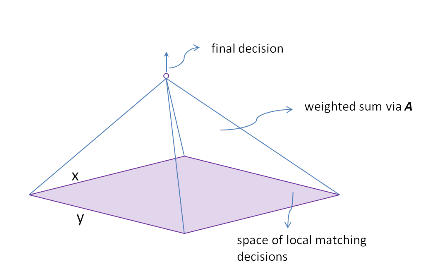
\includegraphics[height=6cm,width=7cm]{bilinear.png}
  \label{fig:bilinear}
  \caption{fig:Architecture for linear matching}
\end{figure}

\subsection{从线性到深度}

以上简单的合成策略可以被延伸到一个深度结构来探究匹配短文本的非线性和层次性。不像文本分类,我们需要匹配文本对,在这里被叫做\textbf{平行文本(parrel text)}。这种新的结构基于以下两个直觉:
\begin{description}
\item[局部性] 局部结构可以通过共现的词对来匹配平行文本的语义。这种局部性不应该阻止两个不同的\footnote{在这里指低层次不匹配}元素在高层次进行匹配,因此模型需要一个混合的结构。
\item[层次性] 决策有不同层次的抽象。局部决策,抓住词义相近的词之间的关系,将会逐层形成最后和全局决策。
\end{description}

\begin{figure}
  \centering
  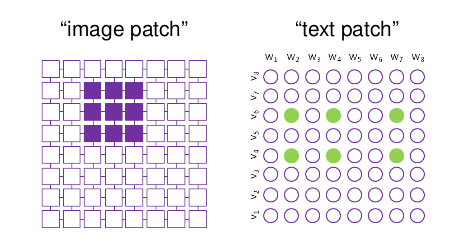
\includegraphics[height=6cm,width=9cm]{imagetext.png}
  \caption{fig:图像块vs文本块}
  \label{fig:patch}
\end{figure}

\subsection{局部性}

文本匹配的局部性问题可以和图像匹配相类比,如图(\ref{fig:patch})所示。大体上说,平行文本的文本块由两个文本之间的关联词决定。像处理图像一样,可以用$(\Omega_{x,p},\Omega_{y,p})$来决定匹配的范围,$(\Omega_{x,p},\Omega_{y,p})$分别代表$X,Y$的子集。“块(patches)”用来获取子集的内在结构。与图像使用长方形来作为块不同的是,文本块不能用给定的连续空间。因为词不一定和其周围词相关,因此需要通过匹配文本的共现对来发现。文章后面用bilingual topic model来发现共现对,这种方法可以成功获取同领域和不同领域的共现对。基本的思想是:1).当词对多次在跨领域出现的时候(例如,感冒——抗体),它们在决定匹配的时候有很高的得分;2).当词对多次在相同领域出现的时候(例如,夏威夷——度假),它们对该领域匹配有很高的帮助。例如,从QA对中就可以发现,夏威夷和RAM就不可能作为一个共现对。也就是说,模型只在块中匹配底层次的语义关系。

\subsection{层次性}

在块中局部决策完成后(他们当中多数都是NULL对于词对来说),这些局部决策会被送到更高层次,这些决策在高层会被混合处理,然后再被送到更高层,直到最后的决策。图(\ref{fig:gao}) 给出了一个层次决策的例子。如其中所示,词对“sightseeing in paris”和“sightseeing in berlin”能够因“sightseeing”来形成一个更高的决策。也能够相对的形成“hotel”和“transportation”,这些都能形成一个更高的层次“travel”。注意到高层次主题对底层次主题没有包含关系。

直觉上,决策过程会有相当大的区别。例如:当联合“sightseeing in paris”和“sightseeing in berlin”时,更像逻辑中的OR因为只有其中的一个是正的。一个更复杂的方法是必要的,例如,“travel”主题需要不止一个元素,像“weather”等等,但是也不是都需要。这样特别的策略可以通过神经元来实现:
\begin{displaymath}
  s_p(x,y) = f(w_p^{T}\Phi_p(x,y))
\end{displaymath}
f是激活函数。这里将具体的函数留给后续章节。

\begin{figure}
  \centering
  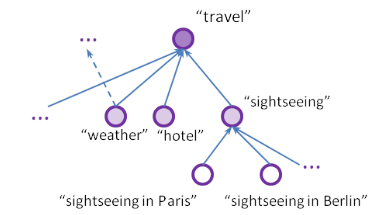
\includegraphics[height=6cm,width=9cm]{gao.png}
  \caption{层次决策}
  \label{fig:gao}
\end{figure}

\section{深层结构的构建}

构建深层结构需要两步:1.给平行文本决定bilingual model;2.根据DNN,构建DAG,描述层次结构。

\subsection{平行文本的主题建模}

该paper利用的方法有点像多语言的PLSI,也就是将平行文本放在一起。对不同领域建立一个不同的词表,避免其混合。例如在领域X出现的hotel和在Y中出现的hotel不应该是一个词。在训练的时候,用LDA+Gibbs sampling。对于X中出现的词,不一定只有单一的领域,假设有$H=\{T_1,\cdots ,T_L\}$这个集合按层次递减。

\subsection{获得匹配结构}

给定主题集合H,deep matching model可以通过三步来获得。
\begin{enumerate}
\item 剪掉在所有主题概率都很低的词。剩下的词在每一个主题确定一个块。
\item 根据H,建立一个DAG G,根据在$T_l 和T_{l-1}$共同出现的词,确定连接。如图(\ref{fig:hir})所示。
\item 重复此过程,建立神经网络。
\end{enumerate}

\begin{figure}
  \centering
  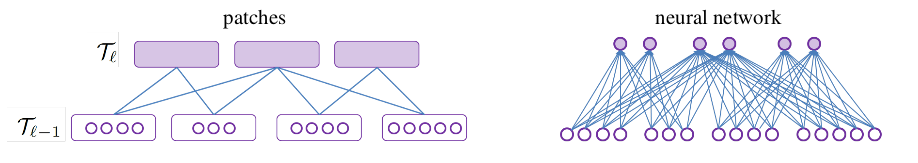
\includegraphics[height=3.5cm,width=14cm]{hir.png}
  \caption{层次神经网络}
  \label{fig:hir}
\end{figure}

具体的网络结构如图(\ref{fig:jiegou})所示。

\begin{figure}
  \centering
  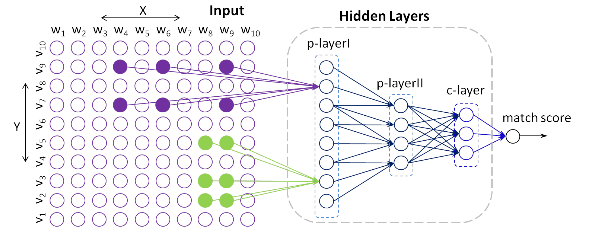
\includegraphics[height=5cm,width=10cm]{jiegou.png}
  \caption{网络结构}
  \label{fig:jiegou}
\end{figure}

\subsection{稀疏性}

这里有两种稀疏性:
\begin{enumerate}
\item 结构本身带来的稀疏性,因为网络中大部分连接都是关闭的。在实验中,仅有2\%的参数是非0的。
\item 第二种稀疏性在于文本的稀疏性,对于实验中,底层只有很小的一部分是有数值的。这是由于两个原因:
  \begin{enumerate}
  \item 平行文本通常很短
  \item 我们就是这么设计的很稀疏的
  \end{enumerate}
  
\end{enumerate}

为了理解稀疏性,下面给出一个定义:

\paragraph{定义}

输入对$(x,y)$有重合块p,当且仅当$x\cap p_x \neq \emptyset 和 y\cap p_y \neq \emptyset$,其中$p_x,p_y$分别是块p在领域$X,Y$的词索引。

在定义重合函数:$\emph{overlap}((x,y),p) = ||p_x \cap x||_0 \cdot || p_y \cap y ||_0 $。提出的架构只允许有重合的部分可以是非0的。更确切的说就是:
\begin{displaymath}
  s_p (x,y) = a_p (x,y) \cdot \emph{overlap} ((x,y),p)
\end{displaymath}
$a_p(x,y)$是激励函数。这种限制对于back-propagation时的tuning非常有用:监督信号(supervision signal)只有在有重合的时候才会被得到。很明显的,如果监督信号在块p停止了,它也不会往下传递给p和p的孩子,即使他们的孩子有其他祖先。也就是说用随机梯度的时候,只需要更新少量节点即可,因而是非常有效率的。\footnote{在这里我的理解就是,因为p已经没有重合的节点了,其他祖先也不需要往这里传了。}

\subsection{局部决策方法}

在隐藏层p-layerI,p-layerII,c-layer,我们允许两种激励函数:
\begin{enumerate}
\item 线性(linear):$f_{lin}(t) = x$
\item sigmoid : $f_{sig} (t) = (1+e^{-t})^{-1}$
\end{enumerate}

在第一层,$(x,y)$的每一个块p有:$M_p = x_p y_p^{T}$;p中第k个局部决策有$a_p^{(k)}(x,y) = f_p^{(k)} (\sum_{n,m}A_{p,nm}^{(k)}M_{p,nm}+b_p^{(k)})$。其中A是权重,f是两种激励函数中的一种。进一步,有:
\begin{displaymath}
  a_p^{(k)}(x,y) = f_p^{(k)} (x_p^{T}L_{x,p}^{(k)}(L_{y,p}^{(k)})y_p+b_p^{(k)})
\end{displaymath}

如图(\ref{fig:jiegou})所示,L是隐藏的二维结构。在输入层之后,二维结构就没有了。也就替换成了,如图(\ref{fig:gongshi})所示的形式。
\begin{figure}
  \centering
  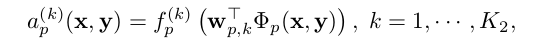
\includegraphics[height=1cm,width=8cm]{gongshi.png}
  \label{fig:gongshi}
\end{figure}
其中$\Phi$是前面所定义的$s_p$。



\end{document}
